\pagestyle{fancy}
\section{Introducción}

AironTools es una empresa mexicana con más de una década de experiencia en la producción y comercialización de herramientas industriales. A lo largo de su trayectoria ha consolidado una base de clientes recurrentes en el sector industrial mécanico y automotriz. Sin embargo, actualmente enfrenta importantes desafíos operativos derivados del uso de procesos manuales y herramientas no integradas para la gestión interna y la atención a clientes.

La gestión de servicios técnicos, inventario, comunicación interna y control de información se realiza mediante hojas de cálculo y formatos físicos, lo que ha derivado en dificultades para la trazabilidad de los servicios, errores en el registro de información, pérdida de datos importantes para la toma de decisiones, y una experiencia limitada para el cliente, al no contar con un sistema que le permita dar seguimiento a sus solicitudes de manera eficiente.

Estas deficiencias afectan directamente la eficiencia operativa, la competitividad y la capacidad de crecimiento de AironTools frente a otras empresas del sector que ya operan con sistemas digitales robustos e interconectados. En este contexto, se propone el diseño e implementación de un sistema de gestión empresarial que permita digitalizar y automatizar los procesos clave de la organización.

El objetivo del proyecto es desarrollar una plataforma integral que centralice la información, mejore la trazabilidad de los servicios ofrecidos, optimice el control de inventario y facilite la comunicación entre las distintas áreas operativas. Este sistema estará alineado con los flujos de trabajo actuales de la empresa, y se construirá bajo una arquitectura escalable que garantice su adaptabilidad y crecimiento a futuro.

Como beneficio, se espera una mejora sustancial en los tiempos de respuesta, una administración más eficiente de los recursos, una atención al cliente más ágil y profesional, y un fortalecimiento de la capacidad competitiva de AironTools en el mercado de herramientas industriales. El presente proyecto se enmarca dentro de la modalidad de experiencia profesional, y responde a una necesidad real detectada en la operación de la empresa.

\section{Justificación}

La propuesta de este proyecto surge de una necesidad concreta identificada en la operación diaria de la empresa AironTools. En la actualidad, la falta de un sistema de gestión empresarial digitalizado ha derivado en múltiples dificultades operativas, entre las que destacan una atención deficiente al cliente, escasa trazabilidad de los servicios técnicos, desorganización en el control de inventario y una gestión interna basada en registros manuales. Esta situación ha limitado significativamente la capacidad de la empresa para escalar sus operaciones y mantenerse competitiva frente a organizaciones del mismo sector que ya han implementado soluciones tecnológicas robustas.

Los registros actuales de clientes, servicios, inventario y empleados se realizan mediante formatos físicos o archivos aislados, lo cual genera errores frecuentes, pérdida de información, duplicidad de datos y demoras en la atención. Estas deficiencias impactan de manera directa en la eficiencia del personal, en la capacidad de respuesta y en la imagen profesional que la empresa proyecta a sus clientes.

Frente a este panorama, la implementación de un sistema de gestión empresarial integral representa una solución estratégica. Este sistema permitirá centralizar en una sola plataforma la información relacionada con empleados, clientes, servicios y productos, lo que facilitará la trazabilidad del flujo de trabajo desde la solicitud de un servicio hasta la entrega final. Además, la automatización de notificaciones y la digitalización de los procesos permitirán establecer una comunicación más eficiente con los clientes, otorgándoles información puntual y transparente sobre el avance de sus solicitudes.

Otra ventaja clave de esta solución es la optimización del control de inventario. A través de funciones como reportes automático, será posible reducir errores, evitar datos faltantes críticos en documentaciones técnicas y anticipar necesidades operativas. A su vez, los reportes generados por el sistema facilitarán la toma de decisiones basadas en datos reales y actualizados, incrementando la capacidad de análisis y planificación de la empresa.

En conjunto, esta propuesta tecnológica contribuirá a mejorar la productividad interna, profesionalizar la operación diaria y elevar la calidad del servicio ofrecido a los clientes. También permitirá documentar formalmente los procesos internos, asegurando su replicabilidad y continuidad. La digitalización de estas funciones no solo responde a una necesidad interna urgente, sino que posiciona a AironTools como una empresa moderna, eficiente y con visión de crecimiento sostenible en un mercado altamente competitivo.

\section{Objetivo general}
Diseñar un sistema digital de gestión empresarial para AironTools que automatice y centralice los procesos internos de atención al cliente, servicios técnicos, control de inventario y comunicación organizacional, con el fin de mejorar la eficiencia operativa, la trazabilidad de los servicios y la calidad del servicio ofrecido.

\section{Objetivos específicos}
\begin{enumerate}
	\item Desarrollar un módulo de gestión de usuarios que permita registrar, organizar y asignar roles diferenciados al personal de AironTools según sus funciones operativas mediante permisos.

	\item Implementar un módulo de gestión de clientes que facilite el registro, seguimiento del historial de atención y mejora en la comunicación con los clientes.

	\item Automatizar el flujo completo de los servicios técnicos, desde el ingreso del equipo hasta su entrega, integrando notificaciones en cada etapa del proceso.

	\item Diseñar un módulo de control de inventario que permita registrar, editar y consultar productos con sus respectivos detalles, funcionando como catálogo actualizado de herramientas.
\end{enumerate}

\section{Trabajos relacionados}

A continuación se presentan seis trabajos que abordan problemáticas similares a las identificadas en el presente proyecto. Se analiza su propósito, contexto, solución implementada y resultados obtenidos, con el fin de establecer un marco de referencia que oriente el diseño del sistema propuesto para AironTools.

\subsection{La gestión empresarial como factor clave de desarrollo de las spin-offs universitarias. Análisis organizativo y financiero \cite{Rodeiro2012}.}

Este artículo académico fue publicado en la revista *Observatorio de la Economía Latinoamericana* por los autores Rodeiro Pazos, Fernández López y Rodríguez González, con el objetivo de analizar el papel que desempeña la gestión empresarial en el desarrollo y consolidación de las spin-offs universitarias en Galicia, España. 

Se atendió el problema del bajo rendimiento y escasa consolidación de estas empresas, considerando que a pesar de surgir en entornos de alta investigación y conocimiento, muchas fracasan por deficiencias en gestión empresarial y financiación. El artículo tiene como finalidad identificar los factores organizativos y financieros que limitan el crecimiento de las spin-offs.

La solución planteada fue un análisis empírico a partir de encuestas aplicadas a responsables de estas empresas, lo cual permitió construir una caracterización organizativa y financiera de las spin-offs. Los resultados mostraron que las principales barreras para su desarrollo son la falta de capacidades en gestión, la escasa experiencia empresarial del equipo fundador, y la limitada estructura financiera, recomendando como acción clave el fortalecimiento de la gestión desde etapas tempranas.


\subsection{Proceso Administrativo y Gestión Empresarial en COPROABAS, Jinotega \cite{Flores15}.}
La tesis titulada “Proceso Administrativo y Gestión Empresarial en COPROABAS, Jinotega 2010-2013” fue elaborada por Silvia Elena Flores Orozco como requisito para optar al título de Maestría en Gerencia Empresarial en la UNAN-FAREM Matagalpa. Este trabajo se enfocó en analizar si la cooperativa aplicaba adecuadamente los conceptos administrativos que permitieran una gestión eficiente. La investigación fue de tipo descriptiva y transversal, apoyada por métodos teóricos y empíricos, con la participación de 15 trabajadores, dos jefes de área y un gerente.

El estudio se desarrolló con base en dos variables principales: el proceso administrativo (planeación, organización, dirección y control) y la gestión empresarial. Se identificó que estas funciones eran ejecutadas parcialmente y que existía una débil estructuración en la organización, ausencia de manuales de funciones y políticas claras, y carencia de una cultura administrativa. Los resultados permitieron proponer alternativas para fortalecer el desempeño organizacional de la cooperativa mediante una mejor aplicación del proceso administrativo y una gestión más profesionalizada.
\subsection{Gestión Empresarial y Desarrollo \cite{Reyes12}.}

Este proyecto de investigación fue elaborado por Giovanni E. Reyes en el marco del Doctorado en Ciencias de la Dirección de la Universidad del Rosario (Colombia). El estudio tiene como finalidad principal analizar la gestión empresarial desde una perspectiva sistémica y estratégica, integrando aspectos internos de las organizaciones, su entorno inmediato y el contexto macroeconómico nacional e internacional.

El problema que aborda gira en torno a la necesidad de comprender y fortalecer la perdurabilidad de las unidades productivas mediante el desarrollo de capacidades estratégicas, innovación, gestión del conocimiento y adaptación funcional a contextos complejos. Para resolverlo, se propone un enfoque investigativo fundamentado en tres niveles de análisis: (i) el ámbito subsistémico de la empresa (estructura interna), (ii) su medio ambiente inmediato (relaciones empresariales, infraestructura, entorno local), y (iii) el entorno amplio (macro social, político, económico y tecnológico).

El proyecto plantea una metodología que incluye metaanálisis, planteamientos conceptuales y estudios empíricos. Como resultado, busca generar modelos referenciales aplicables al análisis de empresas, articulando teoría con recomendaciones prácticas, y enfatizando el desarrollo humano sostenible, sustentable y equitativo como finalidad última de la gestión empresarial.

Las similitudes y diferencias con el proyecto propuesto, se presentan en la Tabla \ref{table:trabajosRelacionados}.

\subsection{Planeación Estratégica y Nuevos Proyectos en Empresa Propia \cite{Patino19}.}
Este proyecto terminal fue desarrollado en la Universidad ICESI como trabajo de grado para la carrera de Economía y Negocios Internacionales. El problema que atendió fue la falta de una estructura organizacional clara y estrategias definidas dentro de una empresa apícola en etapa inicial llamada Kopec S.A.S., cuya actividad principal es la producción y comercialización de apitoxina (veneno de abeja) con fines medicinales y cosméticos.

El objetivo principal fue consolidar una propuesta de planeación estratégica para dicha empresa que permitiera establecer su misión, visión, valores y objetivos estratégicos. Para lograrlo, el autor realizó una revisión teórica de modelos reconocidos de planeación estratégica (como los de Newman, Lambert, Colón y Rodríguez, entre otros), así como el uso de herramientas como el análisis FODA y el modelo Canvas.

Como resultado, se diseñó un plan estratégico inicial acompañado de proyecciones financieras y diagnósticos organizacionales que buscan orientar el desarrollo y crecimiento competitivo de Kopec S.A.S. en el mercado apícola colombiano.

Esta investigación abordó la desconexión entre áreas de atención al cliente y los procesos internos de las empresas. Su objetivo fue identificar cómo los sistemas digitales integrados pueden mejorar la experiencia del usuario. Se desarrolló una plataforma que unificaba seguimiento de servicios, notificaciones y canales de contacto. Como resultado, se observó un aumento en la fidelización y satisfacción del cliente.

\begin{longtable}{m{.05\paperwidth} *{2}{m{.33\paperwidth}} @{}}
	\caption{Comparación cualitativa de los trabajos relacionados con el proyecto.}
	\label{table:trabajosRelacionados}\\
	\hline
	\textbf{Ref.} & \textbf{Similitudes} & \textbf{Diferencias} \\
	\hline
	\endfirsthead
	
	\multicolumn{3}{c}{\textbf{Continuación de la Tabla \ref{table:trabajosRelacionados}}} \\
	\hline
	\textbf{Ref.} & \textbf{Similitudes} & \textbf{Diferencias} \\
	\hline
	\endhead
	\hline
	\endlastfoot
	
	\cite{Rodeiro2012} &
\begin{itemize}[topsep=0pt,itemsep=0pt,parsep=0pt,partopsep=0pt,leftmargin=*]
	\item Ambos trabajos reconocen la importancia de la gestión empresarial como clave para la sostenibilidad y crecimiento organizacional.
	\item Se abordan barreras estructurales y organizativas que deben atenderse para mejorar el desempeño de una empresa.
	\item Se destaca la necesidad de fortalecer procesos de gestión desde etapas tempranas del desarrollo empresarial.
\end{itemize} &
\begin{itemize}[topsep=0pt,itemsep=0pt,parsep=0pt,partopsep=0pt,leftmargin=*]
	\item El artículo se centra en el análisis de spin-offs universitarias mediante encuestas y datos estadísticos, mientras que en mi proyecto se desarrolla e implementa una solución tecnológica real en una empresa del sector industrial.
	\item En el trabajo analizado se identifican debilidades en capacidades administrativas, mientras que en mi proyecto se crean herramientas específicas para solucionar dichas deficiencias, como módulos de control, automatización, reportes y trazabilidad.
	\item El artículo propone recomendaciones generales sobre gestión y financiación; en cambio, mi propuesta incluye la integración de tecnologías como NestJS, React, MongoDB y despliegue en AWS.
\end{itemize} \\
\midrule
	
	\cite{Flores15} &
	\begin{itemize}[topsep=0pt,itemsep=0pt,parsep=0pt,partopsep=0pt,leftmargin=*]
		\item Ambos trabajos analizan los elementos del proceso administrativo (planeación, organización, dirección y control).
		\item Se busca fortalecer la gestión empresarial para mejorar el desempeño y sostenibilidad de la organización.
		\item Se identifican problemas derivados de una gestión deficiente y se proponen alternativas de solución.
	\end{itemize} &
	\begin{itemize}[topsep=0pt,itemsep=0pt,parsep=0pt,partopsep=0pt,leftmargin=*]
		\item La tesis se basa en un análisis cualitativo, mientras que mi proyecto desarrolla una solución digital implementada en una empresa real.
		\item Mi trabajo aplica tecnologías modernas como NestJS, React y MongoDB, en contraste con el enfoque tradicional de evaluación administrativa.
		\item La propuesta planteada en mi proyecto incluye automatización, trazabilidad y comunicación digital, aspectos ausentes en el trabajo de Flores.
	\end{itemize} \\
	\midrule
	
	\cite{Reyes12} &
	\begin{itemize}[topsep=0pt,itemsep=0pt,parsep=0pt,partopsep=0pt,leftmargin=*]
		\item Ambos trabajos abordan la gestión empresarial como medio para mejorar el desempeño organizacional.
		\item Reconocen la importancia de factores internos, del entorno inmediato y del contexto macroeconómico.
		\item Promueven la integración de capacidades humanas, innovación y sostenibilidad para lograr organizaciones más eficientes.
	\end{itemize} &
	\begin{itemize}[topsep=0pt,itemsep=0pt,parsep=0pt,partopsep=0pt,leftmargin=*]
		\item El proyecto de Reyes es de tipo académico-conceptual, mientras que el tuyo es una solución aplicada y funcional implementada en una empresa real.
		\item Tu proyecto utiliza herramientas tecnológicas específicas (NestJS, React, MongoDB), mientras que el de Reyes se mantiene en el plano teórico sin desarrollo de software.
		\item El enfoque del proyecto de Reyes está centrado en el desarrollo humano y la inclusión social, mientras que el tuyo se enfoca en la eficiencia operativa y trazabilidad empresarial.
	\end{itemize} \\
	\midrule
	
	\cite{Patino19} &
    \begin{itemize}[topsep=0pt,itemsep=0pt,parsep=0pt,partopsep=0pt,leftmargin=*]
        \item Ambos proyectos se desarrollaron para resolver una problemática empresarial real.
        \item Ambos utilizan principios de planeación estratégica para estructurar el funcionamiento de una organización.
        \item Se enfocan en mejorar la eficiencia operativa y competitividad de una empresa.
    \end{itemize} &
    \begin{itemize}[topsep=0pt,itemsep=0pt,parsep=0pt,partopsep=0pt,leftmargin=*]
        \item El proyecto de Kopec S.A.S. se basa en estrategias organizacionales, mientras que el de AironTools implementa una solución tecnológica concreta.
        \item El trabajo de Kopec no contempla desarrollo de software ni arquitectura técnica; AironTools desarrolla un sistema digital completo.
        \item El proyecto de AironTools incluye infraestructura DevOps, IA y soporte multitenant, aspectos ausentes en Kopec.
    \end{itemize} \\
	\bottomrule
	\end{longtable}
	

\section{Descripción técnica}

El sistema propuesto para AironTools es una aplicación web de gestión empresarial compuesta por módulos funcionales independientes que automatizan y centralizan los procesos clave de la organización. Está orientado a mejorar la atención al cliente, la administración de servicios técnicos, el control de productos y la coordinación interna. Todos los módulos interactúan bajo una arquitectura escalable y mantenible, permitiendo su crecimiento progresivo.

\subsection*{Arquitectura general del sistema}

El sistema sigue una arquitectura modular cliente-servidor, donde el backend y el frontend se desarrollan de forma desacoplada. La comunicación entre ambos se realiza mediante APIs RESTful. Esta estructura permite una mayor flexibilidad, mantenibilidad y facilidad de integración futura con nuevas funcionalidades.

La Figura~\ref{fig:arquitectura} muestra una vista general de la arquitectura del sistema con sus principales componentes.

\begin{figure}[H]
	\centering
	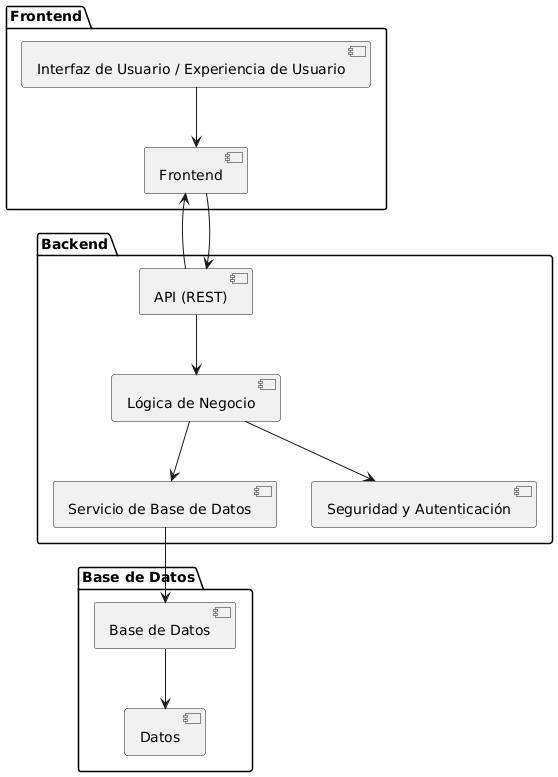
\includegraphics[width=0.9\textwidth]{sistema.png}
	\caption{Arquitectura general del sistema propuesto para AironTools.}
	\label{fig:arquitectura}
\end{figure}

\subsection*{Módulo de usuarios y roles}

Este módulo permite registrar empleados, asignar roles diferenciados y gestionar permisos de acceso al sistema. Incluye funcionalidades de autenticación y autorización para garantizar la seguridad del sistema, además de una interfaz de administración para el rol de superadministrador.

\subsection*{Módulo de clientes}

Permite registrar tanto a clientes individuales como a empresas, asociando datos de contacto e historial de servicios recibidos. Este módulo se integra con el sistema de notificaciones para mantener informados a los clientes durante cada etapa del servicio técnico.

\subsection*{Módulo de servicios técnicos}

Automatiza el flujo completo de atención a servicios como reparación, mantenimiento, demostración y cotización. El sistema registra desde el ingreso del equipo hasta su diagnóstico, reparación, validación final y entrega al cliente. Se incluyen notificaciones automáticas por cambios de estado.

\begin{figure}[H]
	\centering
	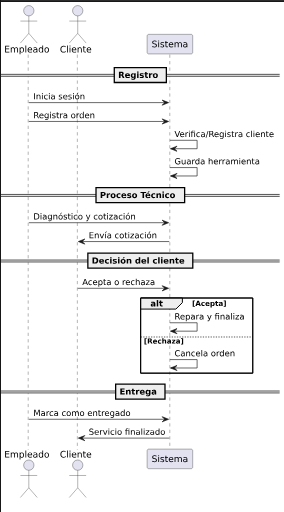
\includegraphics[width=0.9\textwidth]{secuencia-sistema.png}
	\caption{Diagrama de secuencia del flujo de atención a servicios técnicos.}
	\label{fig:secuencia}
\end{figure}

\begin{figure}[H]
	\centering
	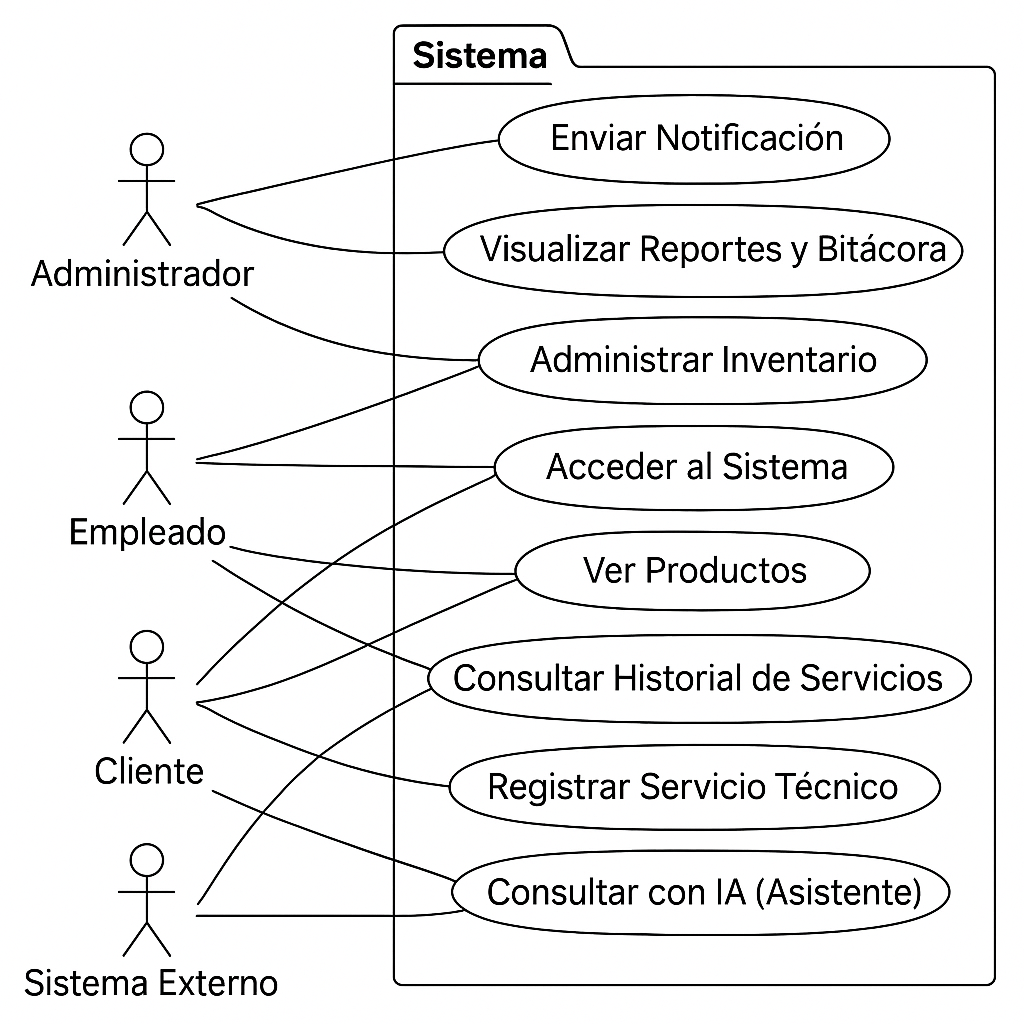
\includegraphics[width=0.9\textwidth]{casos-uso-sistema.png}
	\caption{Diagrama de casos de uso asociados a los módulos funcionales del sistema.}
	\label{fig:casosuso}
\end{figure}

\subsection*{Módulo de productos}

Este módulo permite registrar, editar y consultar productos e insumos disponibles para la venta o uso interno. Los productos se organizan jerárquicamente en familias, categorías y subcategorías, con información como nombre, precio, descripción, imágenes y diagramas técnicos. Actualmente funciona como un catálogo visual centralizado, integrable con los servicios y clientes.

\subsection*{Módulo de notificaciones y comunicación interna}

El sistema integra notificaciones por correo electrónico según el estado del servicio. También se contempla un sistema básico de comunicación en tiempo real mediante WebSockets para uso interno entre áreas operativas, con opción de extenderse a chat interno completo.

\subsection*{Resumen visual de módulos e interacciones}

La Figura~\ref{fig:modulos} muestra un esquema visual de los módulos implementados y cómo se comunican entre sí para cumplir con los objetivos del sistema.

\begin{figure}[H]
	\centering
	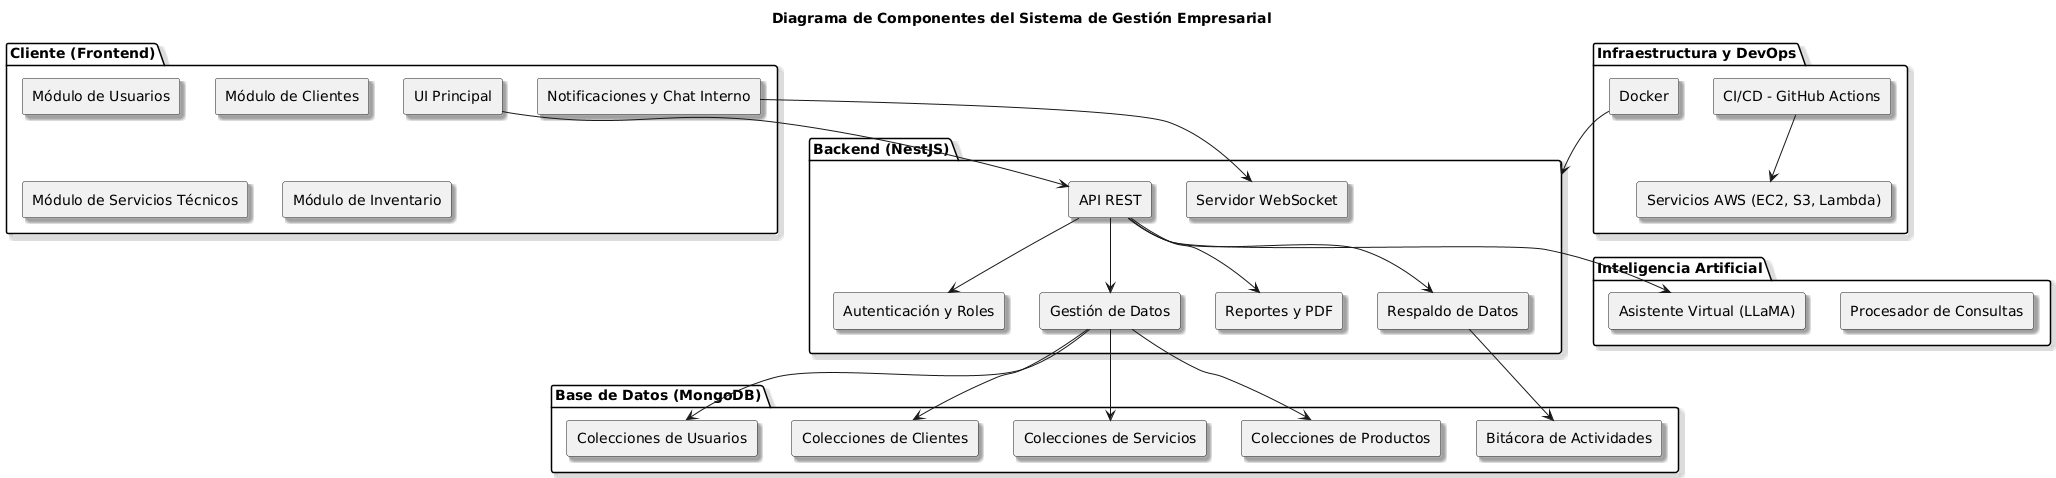
\includegraphics[width=0.9\textwidth]{componentes-sistema.png}
	\caption{Módulos principales del sistema de gestión y sus interacciones.}
	\label{fig:modulos}
\end{figure}

	
\section{Especificación técnica}

El sistema será accesible mediante una aplicación web dividida en backend y frontend independientes. Los módulos funcionales operan de forma integrada a través de APIs RESTful, alineados con los flujos reales de la empresa. La arquitectura es modular, escalable y mantenible.

\subsection*{Tecnologías utilizadas}

\begin{itemize}
	\item \textbf{Backend:} NestJS con TypeScript sobre Node.js. Arquitectura modular compuesta por controladores, servicios, repositorios, DTOs y validaciones centralizadas usando \texttt{class-validator}. Esta estructura permite separar responsabilidades y mantener el sistema escalable y mantenible.
	\item \textbf{Frontend:} React.js con TypeScript. Arquitectura basada en \textbf{Screaming Architecture} y \textbf{Clean Architecture}, lo cual permite que la estructura del proyecto refleje claramente sus funcionalidades, promoviendo una alta cohesión y bajo acoplamiento entre componentes.
	\item \textbf{Base de datos:} MongoDB, con soporte para múltiples empresas (multitenant) mediante aislamiento lógico de datos.
	\item \textbf{Interfaz de usuario:} HTML5 y CSS3, apoyado con Figma para diseño de prototipos y TalwindCSS para componentes accesibles y responsivos.
	\item \textbf{Comunicación:} WebSockets para mensajería interna en tiempo real y actualizaciones automáticas de estados.
	\item \textbf{Correo electrónico:} Protocolo SMTP para el envío automático de notificaciones operativas a usuarios internos y clientes.
	\item \textbf{Control de versiones e integración continua:} Git para versionamiento y GitHub Actions para automatización del pipeline CI/CD.
	\item \textbf{Contenerización y despliegue:} Uso de Docker para encapsular servicios, con despliegue en AWS (EC2 para la aplicación, S3 para archivos y Lambda para procesos automatizados).
\end{itemize}


\subsection*{Alcance funcional}

El proyecto contempla como mínimo la implementación de los siguientes módulos:

\begin{itemize}
	\item Gestión de empleados con autenticación y roles.
	\item Registro y administración de clientes individuales y empresariales.
	\item Flujo completo de servicios técnicos con seguimiento automatizado.
	\item Catálogo digital de productos e insumos.
	\item Notificaciones por correo y sistema de comunicación interna.
	\item Respaldo automático configurable y generación de reportes técnicos.
	\item Soporte multitenant para múltiples compañías, según la empresa seleccionada al iniciar sesión.
\end{itemize}

\subsection*{Criterios de finalización}

El sistema se considerará funcional cuando:

\begin{itemize}
	\item Cada módulo esté implementado y probado funcionalmente.
	\item Los casos de uso estén validados y documentados.
	\item El sistema esté desplegado en un entorno de pruebas funcional.
	\item Se incluya documentación técnica, manual de usuario y código fuente organizado.
	\item Se entregue una carpeta digital con el PDF final, código fuente comprimido y apéndices con el listado de código.
\end{itemize}


	
	Cada módulo será considerado finalizado cuando cumpla con los casos de uso definidos, haya sido probado funcionalmente y esté debidamente documentado. Además, el sistema deberá encontrarse desplegado en un entorno de pruebas funcional para su demostración.
	
	La Figura~\ref{fig:modulos} muestra un esquema general de los módulos definidos, y la Figura~\ref{fig:casosuso} representa los principales casos de uso considerados para la validación del sistema.
	
	\vspace{0.5cm}
	
	%Este texto SÍ debe incluirse para que la propuesta pueda ser aceptada.
	Al concluir el proyecto de integración se entregará a la Coordinación de Estudios de Ingeniería en Computación una carpeta digital que incluirá el reporte final del proyecto en un archivo PDF (sin restricciones)\footnote{Debe poder visualizarse sin solicitar contraseña}, el código fuente del proyecto en un archivo comprimido (sin restricciones)\footnote{Debe poder descomprimirse sin solicitar contraseña}. Además, la sección de apéndices del reporte final contendrá al menos un listado del código fuente desarrollado.


	\section{Calendario de actividades}

Las actividades a realizar durante el Trimestre 2025-Invierno en la UEA Proyecto de Integración de Ingeniería en Computación I (clave 1100113), con un valor de 18 créditos y una duración total de 198 horas, se presentan en la Tabla~\ref{table:calendarioActividades}.

\begin{longtable}{p{0.05\textwidth} p{0.4\textwidth} p{0.1\textwidth} p{0.35\textwidth}}
	\caption{Listado de actividades a realizar durante el Trimestre 2025-Invierno.}
  	\label{table:calendarioActividades}\\
	\toprule
	\textbf{No.} & \textbf{Actividad} & \textbf{Horas} & \textbf{Entregable} \\
	\hline
	\endfirsthead

	\multicolumn{4}{c}{\textbf{Continuación de la Tabla \ref{table:calendarioActividades}}}\\
	\hline
	\textbf{No.} & \textbf{Actividad} & \textbf{Horas} & \textbf{Entregable} \\
	\hline
	\endhead

	\hline
	\endlastfoot

	1 & Levantamiento de requerimientos y análisis del sistema actual en AironTools. & 20 & Documento de requerimientos \\
	\midrule

	2 & Diseño de arquitectura del sistema y definición de módulos. & 20 & Diagramas de arquitectura y diseño técnico \\
	\midrule

	3 & Desarrollo del módulo de autenticación y gestión de usuarios. & 25 & Módulo funcional con control de acceso y roles \\
	\midrule

	4 & Desarrollo del módulo de gestión de clientes. & 20 & Registro, historial y vista de clientes implementados \\
	\midrule

	5 & Desarrollo del módulo de servicios técnicos (flujo completo). & 25 & Módulo de flujo de servicio técnico automatizado \\
	\midrule

	6 & Desarrollo del módulo de inventario. & 20 & Registro, movimientos y alertas de inventario \\
	\midrule

	7 & Implementación de sistema de notificaciones y comunicación interna. & 20 & Notificaciones por correo, alertas internas y tareas asignadas \\
	\midrule

	8 & Pruebas funcionales e integración de los módulos. & 20 & Reporte de pruebas, casos de uso validados \\
	\midrule

	9 & Despliegue en entorno de pruebas y revisión técnica. & 15 & Sistema desplegado en servidor y documentación preliminar \\
	\midrule

	10 & Documentación técnica y elaboración de manual de usuario. & 13 & Manual de usuario, guía de instalación y documentación del sistema \\
	\bottomrule
\end{longtable}

\footnotetext{La planeación cubre el análisis, diseño, desarrollo, pruebas, despliegue y documentación del sistema, abarcando las 198 horas correspondientes a la UEA mencionada.}




\section{Factibilidad técnica y operativa}

\subsection{Factibilidad técnica}

El proyecto de desarrollo del sistema de gestión empresarial para AironTools es técnicamente viable, ya que el responsable del desarrollo cuenta con los conocimientos y habilidades necesarios para implementar los módulos definidos en el tiempo estipulado. Entre las competencias destacadas se encuentran:

\begin{itemize}
	\item Conocimientos avanzados en desarrollo web fullstack utilizando tecnologías como React.js, TypeScript y NestJS.
	\item Experiencia en diseño e implementación de arquitecturas modulares y sistemas empresariales.
	\item Habilidad en pruebas, documentación técnica y despliegue de sistemas.
\end{itemize}

Los recursos disponibles para el desarrollo y pruebas del sistema son los siguientes:

\begin{itemize}
	\item Equipos de cómputo con procesadores Intel Core i7, 16 GB de RAM y almacenamiento SSD.
	\item Acceso a entornos locales y servidores remotos para pruebas y despliegue del sistema.
	\item Conectividad de red estable para realizar pruebas multiusuario y simulaciones reales.
\end{itemize}

Las herramientas que se utilizarán durante el desarrollo incluyen:

\begin{itemize}
	\item \textbf{Frontend:} React.js con TypeScript, Figma para prototipado, y TalwindCSS para diseño de interfaz.
	\item \textbf{Backend:} NestJS con Node.js y MongoDB como base de datos.
	\item \textbf{Control de versiones:} Git y GitHub.
	\item \textbf{Contenedores y despliegue:} Docker, GitHub Actions para integración y entrega continua.
\end{itemize}

No se requieren recursos físicos adicionales ni licencias de software especiales, ya que todas las herramientas son de uso libre o ya están disponibles.

\subsection{Factibilidad operativa}

El sistema propuesto presenta una alta factibilidad operativa dentro de la empresa AironTools, por las siguientes razones:

\begin{itemize}
	\item \textbf{Adaptabilidad a los procesos actuales:} El sistema está alineado con los flujos de trabajo reales de la empresa, por lo que su adopción no requerirá una reestructuración significativa.
	
	\item \textbf{Aceptación organizacional:} El proyecto cuenta con el respaldo directo del jefe de área, el Ing. Víctor Benjamín Aguilar Orocio, responsable de la implementación en la empresa.
	
	\item \textbf{Capacitación del personal:} Se prevé una estrategia de introducción y formación progresiva, asegurando que los empleados comprendan y utilicen el sistema eficazmente.
	
	\item \textbf{Facilidad de uso y soporte:} La interfaz estará diseñada con criterios de usabilidad, y el sistema incluirá funciones de ayuda y comunicación interna que facilitarán su soporte continuo.
	
	\item \textbf{Extensibilidad y mantenimiento:} Gracias a su arquitectura modular, el sistema podrá adaptarse a futuras necesidades o integrarse con nuevas tecnologías sin comprometer su estabilidad.
\end{itemize}

\vspace{0.5cm}
\section{Estimación de costos}

La presente sección muestra una estimación comercial del capital necesario para el desarrollo del sistema de gestión empresarial propuesto, considerando tanto los recursos técnicos como el valor del trabajo intelectual involucrado. Se han incluido costos asociados a infraestructura, herramientas, servicios y personal. Esta estimación representa una aproximación realista en caso de que el proyecto se desee escalar o comercializar.

La estimación de costos del proyecto se presenta en la Tabla~\ref{table:tablaCostos}.

\begin{longtable}{m{6.5cm} m{4.5cm} m{4cm}}
	\caption{Estimación de costos del proyecto.}
  	\label{table:tablaCostos}\\
  	\toprule
	\textbf{Descripción} & \textbf{Costo unitario (MXN)} & \textbf{Costo total (MXN)} \\
	\hline
	\endfirsthead

	\multicolumn{3}{c}{\textbf{Continuación de la Tabla \ref{table:tablaCostos}}}\\
	\hline
	\textbf{Descripción} & \textbf{Costo unitario (MXN)} & \textbf{Costo total (MXN)} \\
	\hline
	\endhead

	\hline
	\endlastfoot

Infraestructura de servidores (entorno de pruebas y producción) & \$3,000.00 $\times$ 1 mes & \$9,000.00 (3 meses) \\
\midrule

Servicios en la nube (almacenamiento, correos, CI/CD) & \$2,000.00 $\times$ 1 mes & \$6,000.00 (3 meses) \\
\midrule

Trabajo de desarrollo (fullstack)~\cite{Desarrollador} & \$25,000.00 $\times$ 1 mes & \$75,000.00 (3 meses) \\
\midrule

Diseño UI/UX y prototipado de interfaces & \$10,000.00 $\times$ 1 mes & \$30,000.00 (3 meses) \\
\midrule

Capacitación y soporte técnico interno & \$5,000.00 $\times$ 1 mes & \$15,000.00 (3 meses) \\
\midrule

Pruebas, validación y documentación & \$4,000.00 $\times$ 1 mes & \$12,000.00 (3 meses) \\
\midrule

\textbf{Costo total estimado} & — & \textbf{\$147,000.00} \\
\bottomrule
\end{longtable}

\footnotetext{Los valores fueron obtenidos con base en referencias de mercado, experiencia previa en proyectos similares y validación con el responsable directo en la empresa. Incluyen costos de infraestructura, servicios, diseño, desarrollo y soporte.}
